%
% Economics of the Quantum Internet
%

\section{Economics of the quantum internet} \index{Economics}

Any form of computation comes at an economic cost, but also brings with it a payoff. A key consideration in any model for computation is the tradeoff between the two. Because the computational power of quantum computers scales inherently differently than classical computers, we expect economic indicators to exhibit different scaling characteristics and dynamics also, thereby fundamentally altering the economic landscape of the post-quantum world.

We will now treat some of these economic issues in the context of a global network of unified quantum computing resources, which are then equitably time-shared\index{Time-sharing}. We argue in Sec.~\ref{sec:quant_ec_lev} that this time-shared model for quantum computation is always more computationally efficient than having distinct quantum computers operating independently in parallel, owing to the super-linear scaling in their joint computational power. While this section provides mathematical details of various economic models, Secs.~\ref{sec:economics} \& \ref{sec:quantcoin} provide a popular, high-level discussion of these issues.

%
% Classical-Equivalent Computational Power & Computational Scaling Functions
%

\subsection{Classical-equivalent computational power \& computational scaling functions}\index{Classical-equivalent computational power}\index{Computational scaling functions}

Let $t$ be the classical-equivalent runtime\index{Classical-equivalent computational power} of a quantum algorithm comprising $n$ qubits -- that is, how long would a given classical computer require to implement this $n$-qubit quantum computation? We define a \textit{computational scaling function}\index{Computational scaling functions} characterising this relationship,

\begin{definition}[Computational scaling functions] \label{def:scaling_func}\index{Computational scaling functions} 
The computational scaling function, $f_\text{sc}$, relates the number of qubits held by a quantum computer, $n$, and the classical-equivalent runtime, $t$, of the algorithm it implements,
\begin{align}
t = f_\text{sc}(n),
\end{align}
	where $f_\text{sc}$ is monotonically increasing, and depends heavily on both the algorithm being implemented, as well as the architecture of the computer.
\end{definition}

The exact form of the scaling function will be specific to the algorithm being deployed\footnote{For example, the \textit{circuit depth}\index{Circuit depth}, i.e number of gate applications in series, will heavily influence the number of classical steps required to simulate the circuit.}, and the computational model (e.g cluster states vs the circuit model, as well as choices in error correction, amongst other factors). Most notably, different quantum algorithms offer different scalings in their quantum speedup -- Grover's algorithm offers only a quadratic quantum speedup, compared to the exponential speedup afforded by Shor's algorithm\index{Shor's algorithm}. Thus, the computational scaling function depends on both the hardware and software, and may therefore differ between different users operating the same computer.

%
% Virtual Scaling Functions
%

\subsubsection{Virtual computational scaling functions}\index{Virtual computational scaling functions}

If a network of quantum computers were combined into a single, larger \textit{virtual quantum computer}\index{Virtual quantum computer} (Sec.~\ref{sec:GVQC}) using a distributed model for quantum computation (Sec.~\ref{sec:dist_QC}), we can define a computational scaling function relationship for the virtual device,

\begin{definition}[Virtual scaling function]\index{Virtual computational scaling functions}
The joint classical-equivalent runtime of a distributed virtual quantum computation over a network is,
\begin{align}
t_\text{joint} = f_\text{sc}^\text{virtual}(n_\text{global}),
\end{align}
where,
\begin{align}
n_\text{global} = \sum_{j\in\text{nodes}} n_j,
\end{align}
is the total number of qubits in the network, with $j$ summing over all nodes in the network, each of which holds $n_j$ qubits. $f_\text{sc}^\text{virtual}$ is obtained from $f_\text{sc}$ by factoring in network overheads and inefficiencies. With perfect network efficiency, \mbox{$f_\text{sc}^\text{virtual}=f_\text{sc}$}.
\end{definition}

%
% Combined Computational Scaling Functions
%

\subsubsection{Combined computational scaling functions}\index{Combined computational scaling functions}\label{sec:comb_comp_sc_func}

Until now we have characterised the entire network by a single scaling function. Of course, the scaling functions observed by different market participants needn't all be the same, as they are functions of not only the hardware, but also the participants' different algorithmic applications (i.e software).

Consider taking a single unit of time (i.e we are ignoring cost discounting\index{Cost discounting} over multiple units of time) and dividing it amongst a number of nodes, $n_\text{nodes}$, each with their own scaling function, $f_\text{sc}^{(i)}$. The total classical-equivalent runtime of the computation is additive, given simply by a linear combination of the classical-equivalent processing times of the individual nodes. This yields the relationship for combining scaling functions,
\begin{definition}[Combined scaling functions]\index{Combined computational scaling functions}\label{def:comb_sc_func}
The effective combined computational scaling function, $f_\text{sc}^\text{(joint)}$, of a group of participants, each with their own scaling functions, $f_\text{sc}^{(i)}$, is given by,
\begin{align}
	t_\text{joint} &= \sum_{i=1}^{n_{\text{nodes}}} \beta_i \cdot f_\text{sc}^{(i)}(n_\text{global}) \nonumber \\
	&= f_\text{sc}^\text{(joint)}(n_\text{global}),
\end{align}
where $\beta_i$ characterise the share of processing time allocated to each node, and for normalisation,
\begin{align}
\sum_{i=1}^{n_\text{nodes}} \beta_i = 1.
\end{align}

\end{definition}

Thus, the joint scaling function of the entire network is simply given by a linear combination (weighted average) of the scaling functions of the different market participants.

%
% Network Price Scaling Factor
%

\subsection{Network price scaling factor}\label{sec:NPSF}\index{Network price scaling factor}

One parameter that appears ubiquitously in the upcoming economic models is the computational power of a quantum computer per qubit. This relates the power and size of the computer. We define this as the \textit{network price scaling factor},

\begin{definition}[Network price scaling factor]\label{def:NPSF}\index{Network price scaling factor}
The network price scaling factor is defined as the computational power per qubit,
\begin{align}
\chi_\text{sc}(n) = \frac{f_\text{sc}(n)}{n}.
\end{align}
\end{definition}

This parameter acts as an overall, network size-dependent price scaling factor on:
\begin{itemize}
\item Quantum computational leverage (Sec.~\ref{sec:quant_ec_lev}).
\item Cost of computation (Sec.~\ref{sec:cost_of_comp}).
\item Time-shared computational power (Sec.~\ref{sec:arb_free_time_share}).
\item Quantum computational leverage (Sec.~\ref{sec:quant_ec_lev}).
\item Forward contracts (Sec.~\ref{sec:for_contr}).
\end{itemize}

This lends itself to the elegant interpretation as a cost multiplier on qubit asset, dividend and derivative prices, which warrants investigation of its scaling characteristics, shown in Fig.~\ref{fig:NPSF}. The key observation is that this scaling factor is constant for classical computing, where the scaling function is linear, but monotonically increasing for any super-linear scaling function. For polynomial scaling functions, it has the effect of reducing the order of the polynomial by one. And for exponential scaling functions, it remains exponential.

\begin{figure}[htb!]\index{Network price scaling factor}
	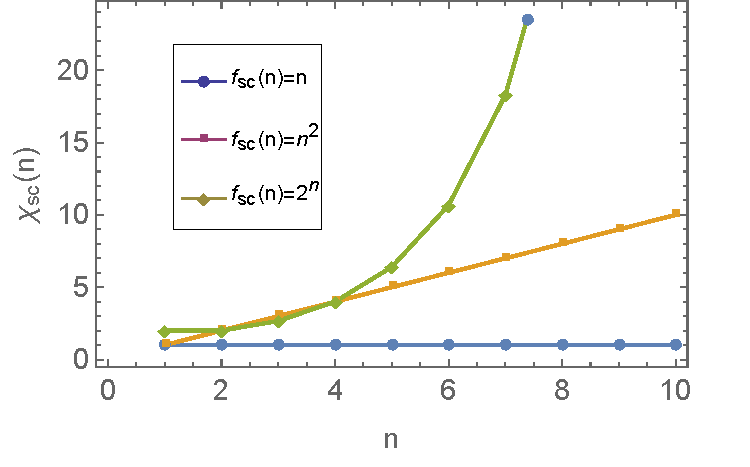
\includegraphics[width=0.47\textwidth]{network_price_scaling_factor}
	\caption{Scaling of the network price scaling factor, $\chi_\text{sc}$, as a function of several representative computational scaling functions, $f_\text{sc}$, where $n$ is network size.} \label{fig:NPSF}
\end{figure}

%
% Economic Model Assumptions
%

\subsection{Economic model assumptions}

Before proceeding with explicit derivations of economic models, we state some assumptions about the dynamics of a marketplace in quantum assets. These assumptions are largely based on historical observations surrounding classical technologies that we might reasonably expect to also apply in the quantum era. However, given that the quantum marketplace is one that hasn't been explored in detail until now, it may be the case that some of these assumptions will require revision. Nonetheless, the general techniques we employ could readily be adapted to some relaxations and variations in these assumptions.

%
% Efficient Markets
%

\subsubsection{Efficient markets}\label{sec:eff_markets} \index{Efficient markets}

We make several assumptions about the efficiency of the quantum marketplace. These are largely based on the conventional efficient-market hypothesis (EMH)\index{Efficient-market hypothesis (EMH)} \cite{???}, readily taught in undergraduate ECON101 and subsequently summarily rejected upon entering ECON202. For ease of exposition, we will remain in the ECON101 classroom.

Some of these assumptions may reasonably turn out to be invalid, or require revision as we learn more about upcoming quantum technologies and the trajectories their marketplace will follow. However, for ease of exposition, and the purposes of presenting some initial rudimentary, \textit{qualitative} analyses and thought experiments, these assumptions simplify our derivations and act as a good starting point for future, more rigorous treatment.

Given that the quantum marketplace doesn't actually exist yet, it isn't immediately clear which assumptions are likely to be valid or not, and future, more sophisticated models will inevitably need to make more appropriate assumptions. Certainly it's no secret that in conventional settings the EMH is flawed in many respects, and some of its idealised assumptions break down in reality.

\begin{postulate}[Efficient markets]\label{post:market_eff}\index{Efficient markets} We make the following efficiency assumptions on the dynamics of the quantum marketplace:
\begin{itemize}
	\item Qubits are a `scarce' resource --- there is always positive, non-zero demand for them.\index{Scarce resource}
	\item No wastage --- quantum computational resources are always fully utilised, with no down-time.\index{Wastage}
	\item Transaction free --- transaction costs are negligible.\index{Transaction cost}
	\item Negligible cost-of-carry --- e.g storage and maintenance costs are negligible.\index{Cost of carry}
	\item High liquidity --- it is always possible to execute transactions at market rates.\index{Liquidity}
	\item Perfect price competition --- there is sufficient competition that profits from quantum hardware and the execution of quantum computations is marginal.\index{Price competition}
	\item Arbitrage-free --- market rates for different assets and derivatives are perfectly consistent, with no opportunity for `free money' by trading on market discrepancies.\index{Arbitrage-free}
	\item Perfect information --- all market participants have complete knowledge of all market variables, including one another.\index{Perfect information}
	\item Rational markets --- all market participants act rationally\footnote{i.e with perfect economic self-interest \latinquote{Avaritia}.} upon available information.\index{Rational markets}
	\item Indefinite asset lifetime --- there is no deterioration or death of quantum hardware over time.\index{Asset lifetime}
	\item There is a risk-free rate of return ($r_\text{rf}$)\index{Risk-free rate of return}
-- the rate of growth exhibited by an investment into an optimal risk-free asset\footnote{Historically these risk-free assets are taken as being US government bonds\index{US government bonds}\index{Risk-free asset}, with the bond yield being the risk-free RoR.}
	\end{itemize}
\end{postulate}

%
% Central Mediating Authority
%

\subsubsection{Central mediating authority}\index{Central mediating authority}

In Secs.~\ref{sec:quant_ec_lev} \& \ref{sec:GVQC} we argue that because of the super-linear scaling in the computational power of networked quantum computers, it will be most economically efficient to unify the world's entire collective quantum computational resources over the network and time-share their joint computational power. For this reason, we will assume that global quantum computing resources are unified, and time-shared equitably (as described in Sec.~\ref{sec:arb_free_time_share}), overseen by a trusted central authority, congruent with our efficient market assumptions (Sec.~\ref{sec:eff_markets}).

However, as discussed in Sec.~\ref{sec:GVQC}, it may be the case that competing strategic interests will drive a wedge between the quantum resources of competitors and adversaries, partitioning them into a set of smaller networks, divided across strategic boundaries. In this instance, the arguments presented in the upcoming sections will apply to these smaller, isolated networks individually.

%
% Network Growth
%

\subsubsection{Network growth} \index{Network growth}

We assume the number of qubits in the global network in the future is growing exponentially over time, i.e the rate of progress of quantum technology will observe a Moore's Law-like behaviour, as with the classical transistor.

This is a reasonable assumption based on the observation of this ubiquitous kind of behaviour in present-day technologies. Classical computing has been on an exponential trajectory since the 1980's, and although it must eventually asymptote, it shows no sign of doing so in the immediate future. Quantum technologies sit at the entry point to this trajectory, and we expect it to continue for the medium-term. Thus, we let the number of qubits in the network be,
\begin{postulate}[Network growth]\label{post:net_growth}\index{Network growth postulate}
The number of qubits in the global quantum internet is growing exponentially over time as,
\begin{align}
	N_t = N_0 {\gamma_N}^{t},
\end{align}
where \mbox{$\gamma_N\geq 1$} characterises the rate of exponential growth in the number of qubits available to the quantum network.
\end{postulate}

The exact value of the growth rate, $\gamma_N$, is obviously unclear at such early stages and will ultimately be determined empirically. Although in the the case of classical computing we have seen a very consistent doubling of computational power roughly every 18 months. This may very well be different for quantum technologies, owing to their fundamentally different engineering requirements (which are much harder in general).

%
% Hardware Cost
%

\subsubsection{Hardware cost} \index{Hardware cost}

Let the dollar cost of physical qubits follow Moore's Law-like dynamics, decreasing exponentially with time,
\begin{postulate}[Hardware cost]\label{post:hardware_cost}\index{Hardware cost}
The dollar-cost of a single physical qubit scales inverse exponentially as,
\begin{align}
	C_t = C_0 {\gamma_C}^{-t},
\end{align}
where \mbox{$\gamma_C\geq 1$} characterises the decay rate.
\end{postulate}

This is consistent with the observed evolution of classical hardware since the beginning of the digital revolution, and it is reasonable to think that technological progress in the quantum era will follow a similar trajectory.

%
% Network Power
%

\subsection{Network power}\index{Network power}\label{sec:network_power}

First and foremost, with a fully interconnected quantum computational network, what is the projection of its net computational power now and into the future? This is simply obtained via the joint computational scaling function applied to projected network size,

\begin{postulate}[Network power]\label{post:network_power}\index{Network power}
The combined computational power of the entire network, measured in FLOPS, is given by,
\begin{align}
P(t) &= f_\text{sc}(n_\text{global})\nonumber \\
&= f_\text{sc}(N_0{\gamma_N}^t).
\end{align}
\end{postulate}

%
% Network Value
%

\subsection{Network value}\index{Network value}\label{sec:network_value}

The simplest economic metric one might define is the collective dollar value of the entire network. That is, the product of the number of qubits on the network and the dollar cost per physical qubit.

\begin{postulate}[Network value]\label{post:network_value}\index{Network value}
The dollar-value of the entire network is given by,
\begin{align}
	V(t) &= C_t N_t \nonumber \\
	&= C_0 N_0 \left(\frac{\gamma_N}{\gamma_C}\right)^t.
\end{align}
\end{postulate}

Note that the collective value of the network appreciates exponentially if the rate of network growth is greater than the rate of decay in the value of physical qubits, otherwise it depreciates. At \mbox{$\gamma_C=\gamma_N$} the network's value remains constant over time. This is shown in Fig.~\ref{fig:network_value}.

\begin{figure}[!htb]
	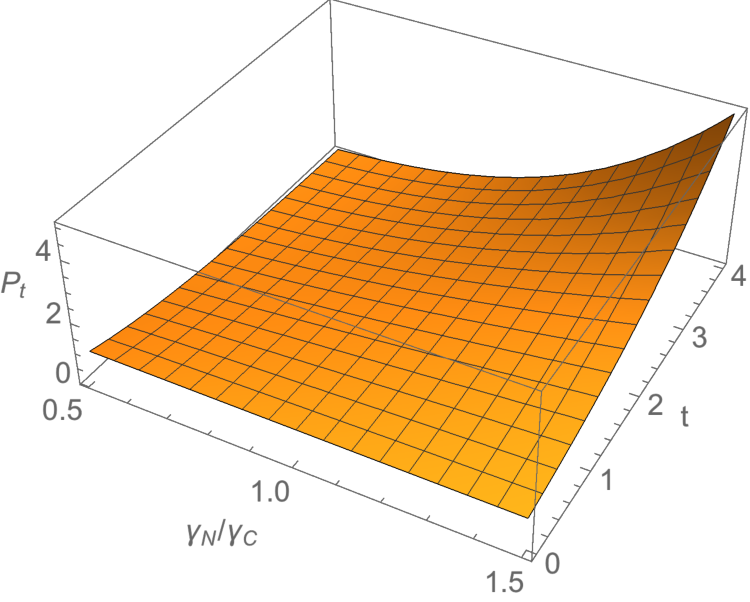
\includegraphics[width=0.4\textwidth]{network_value}
	\caption{Dollar value (in units of \mbox{$C_0N_0$}) of the network as a function of time, growth rate in the number of physical qubits, and rate of decay in the dollar value of physical qubits. When \mbox{$\gamma_N/\gamma_C=1$} the network's value remains constant over time. Above this the network's value appreciates exponentially, and below which it depreciates exponentially against time.} \label{fig:network_value}
\end{figure}

%
% Rate of Return
%

\subsection{Rate of return}\index{Rate of return}

The execution of computations typically has monetary value to the consumer. After all, they are paying hard-earned money for access to the technology!

Suppose the owners of the quantum hardware are not running computations themselves, but rather are collectively licensing out their joint compute-time to end-users. The hardware owners will of course be demanding a profit from their enterprise. The rate at which they earn back their investment into hardware via the licensing of compute-time, we will refer to as the rate of return (RoR), $\gamma_\text{ror}$. We define this as,

\begin{postulate}[Rate of return]\label{post:RoR}\index{Rate of return}
The RoR is defined as,
\begin{align}
e^{\gamma_\text{ror}} = \frac{n_\text{return}}{n_\text{cost}},
\end{align}
where $n_\text{return}$ is the profit made by licensing out the network's joint compute-power for a single unit of time, given a present-day network value of $n_\text{cost}$.
\end{postulate}

A higher $\gamma_\text{ror}$ implies a faster payback on hardware investment\footnote{We have parameterised the RoR as an exponential for convenience when performing derivations with compounding.}.

In an ideal market, where hardware cost is completely predictable, e.g perfectly follows the hardware cost model (Pos.~\ref{post:hardware_cost}), the risk asymptotes to zero and perfect arbitrage (Pos.~\ref{post:market_eff}) will drive the RoR to asymptote to the risk-free RoR, \mbox{$\gamma_\text{ror} \to r_\text{rf}$}. Of course, real markets necessarily exhibit risks and uncertainties, and the RoR on quantum hardware will never be truly risk-free, meaning that upon trading off risk for return, we will always observe \mbox{$\gamma_\text{ror} > r_\text{rf}$}.

%
% Cost Of Computation
%

\subsection{Cost of computation}\label{sec:cost_of_comp} \index{Cost of computation}

In the same scenario as before, where compute-time is being licensed out to end-users, the hardware owners return over a single unit of time equates to the cost of computation over that period.

Let $L_t$ be the dollar-value of utilising the network's computing resources for a single unit of time. This is obtained as the return made on the value of the network per FLOP,
\begin{postulate}[Cost of computation]\label{post:cost_comp}
The efficient-market dollar-value of a computation for a single unit of time, per FLOP is,
\begin{align}\index{Cost of computation postulate}
	L(t) &= \frac{e^{\gamma_\text{ror}} P(t)}{V(t)} \nonumber\\
	&= \frac{e^{\gamma_\text{ror}} C_0{\gamma_C}^{-t}}{\chi_\text{sc}(N_0 {\gamma_N}^t)},
\end{align}
\end{postulate}
which implies,
\begin{postulate}[Spot price of computation]\index{Spot price of computation} The present-day (\mbox{$t=0$}) spot price of a computation per FLOP is,
\begin{align}
L(0) = \frac{e^{\gamma_\text{ror}}C_0}{\chi_\text{sc}(N_0)}.	
\end{align}
\end{postulate}
That is, the value of computations simply approximates the return on initial hardware investment, scaled by its initial computational power, as is intuitively expected.

Note that if $f_\text{sc}$ scales linearly, as per classical computation, we observe a regular exponential decay in the cost of computation, consistent with the classical Moore's Law. On the opposing extreme, for exponentially quantum-enhanced $f_\text{sc}$, the cost of computation decreases super-exponentially with time, an economic behaviour unique to post-classical computation with no classical analogue.

The time-derivative of the cost of computation is strictly negative, assuming correctness of the growth and cost postulates (Pos.~\ref{post:net_growth} \& \ref{post:cost_comp}),
\begin{align}
\frac{\partial L}{\partial t} \leq 0,	
\end{align}
which implies monotonic reduction in the cost of computation over time, unless network growth and cost completely freeze (\mbox{$\gamma_N=\gamma_C=0$}), in which case the cost of computation remains flat.

Examples of the temporal dynamics of the cost of computation are shown in Fig.~\ref{fig:econ_cost_of_comp}.

\begin{figure}[!htb]
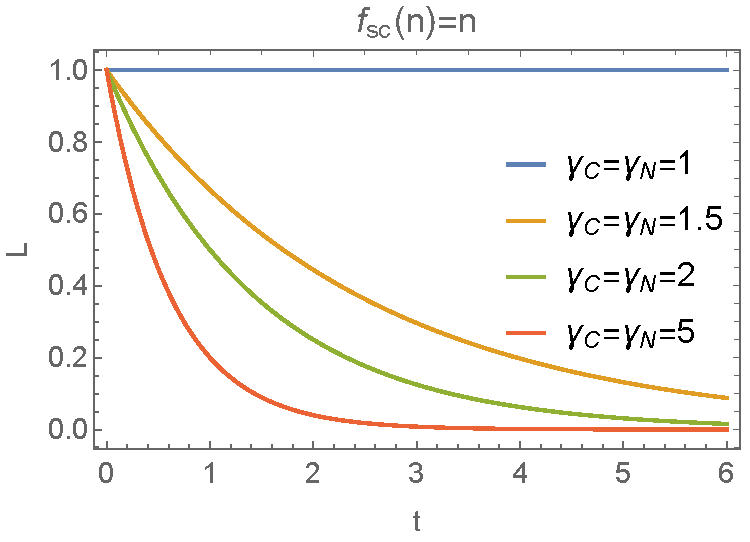
\includegraphics[width=0.4\textwidth]{cost_of_comp_n} \\
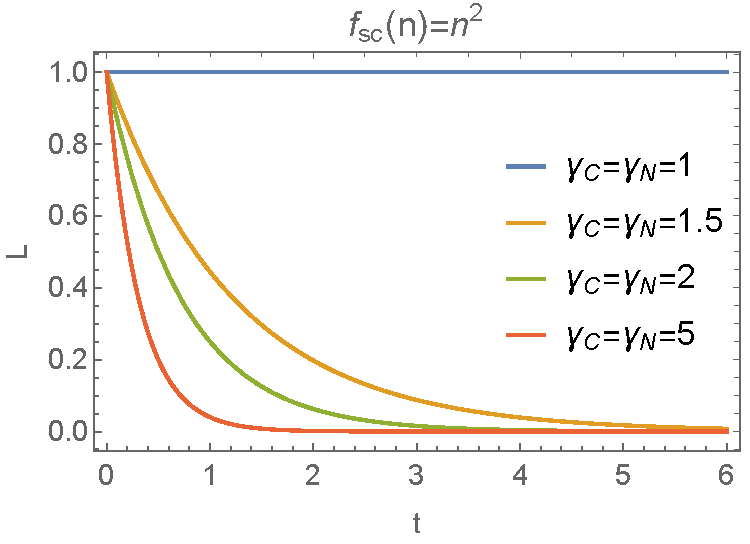
\includegraphics[width=0.4\textwidth]{cost_of_comp_n2} \\
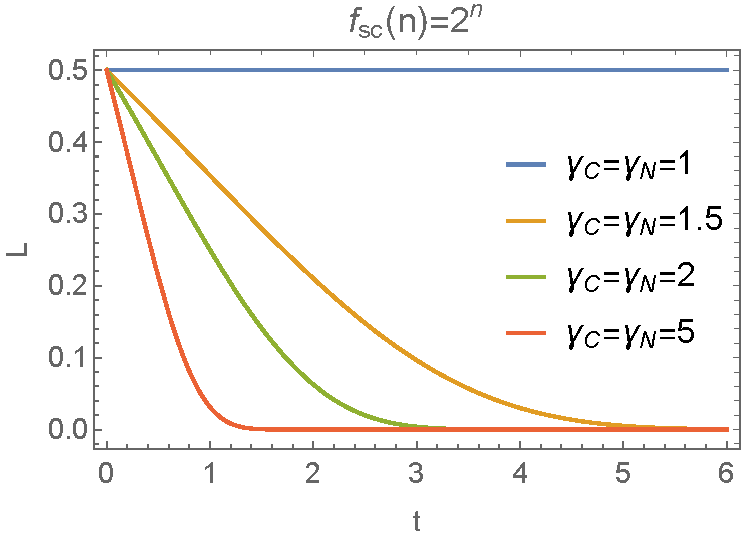
\includegraphics[width=0.4\textwidth]{cost_of_comp_2n}
\caption{Examples of the temporal dynamics of the cost of computation for different scaling functions and exponential growth rates. Units are \mbox{$C_0=N_0=n=1$}, with RoR \mbox{$\gamma_\text{ror}=0$}.}\label{fig:econ_cost_of_comp}
\end{figure}

%
% Arbitrage-Free Time-Sharing
%

\subsection{Arbitrage-free time-sharing model}\label{sec:arb_free_time_share} \index{Arbitrage-free time-sharing model}\index{Time-sharing}

In the context of our global network of unified quantum computers, how do we fairly and equitably allocate time-shares between contributors? We now derive an elementary arbitrage-free model for equitable time-sharing in such a network.

Let,
\begin{align}
	0\leq r_n \leq 1,
\end{align}
be the proportion of compute-time allocated to a node in possession of $n$ qubits, in a global network of $n_\text{global}$ qubits. Arbitrage in the value of physical qubits will enforce the linearity constraint,
\begin{align}
	r_{n_1+n_2} = r_{n_1} + r_{n_2}.
\end{align}
This constraint effectively mandates that `all qubits are created equal', and two qubits are twice as valuable as one \latinquote{Qubit aequalitatem}. Were, for example, a bundle of two qubits more expensive than two individual qubits purchased in isolation, a market participant could perform arbitrage and unfairly gain free compute-time by buying two qubits separately, unifying them, selling the bundle, buying them back individually, and repeating indefinitely until he seizes the entire network.

Additionally, we have assumed no compute-cycles are wasted -- compute-time is always fully utilised, as per Pos.~\ref{post:market_eff}. Then it follows that the time-share of the combined resources of the entire network should be unity,
\begin{align}
	r_{n_\text{global}}=1.
\end{align}
\mbox{$r_{n_\text{global}}<1$} would imply inefficiency via wasted clock-cycles. Combining this with the linearity constraint implies the arbitrage-free time-sharing model,
\begin{definition}[Arbitrage-free time-sharing model] \label{def:arb_free_ts}\index{Arbitrage-free time-sharing model}
In an efficient market for unified quantum computing time-shares\index{Time-sharing}, a network participant in possession of $n$ of the entire $n_\text{global}$ qubits in the network is entitled to the fraction of unified network compute time,
\begin{align}\index{Time-shared compute-time}
	r_n = \frac{n}{n_\text{global}},
\end{align}
where,
\begin{align}
n_\text{global} = \sum_{j\in\text{nodes}} n_j,
\end{align}
is the total number of qubits in the network, and,
\begin{align}
0\leq r_n \leq 1.	
\end{align}
\mbox{$r_n=1$} iff the node has a complete monopoly over qubits, i.e \mbox{$n=n_\text{global}$}.
\end{definition}

Based on this equitable model for time-sharing,
\begin{definition}[Time-shared computing power]\index{Time-shared computing power}
The computing power allocated to each user under the arbitrage-free time-sharing model is,
\begin{align}
	c_n &= r_n \cdot f_\text{sc}(n_\text{global}) \nonumber \\
	&= n \cdot \chi_\text{sc}(n_\text{global}).
\end{align}
\end{definition}

This model is intuitively unsurprising, since it is analogous to the case of classical computer clusters -- nodes receive a time-share proportional to the proportion of the hardware they are contributing to the network. However, it is important to point out that the arbitrage is taking place in the cost of physical qubits, but not in terms of the dollar value of their classical-equivalent processing power, since this is in general non-linearly related to the number of qubits. Arbitrage in computational power per se is complicated by the fact that it is a non-fungible asset that cannot be directly traded, or uniquely associated with a tangible, tradable asset -- its computational value is a function of other assets.

%
% Quantum Computational Leverage
%

\subsection{Quantum computational leverage}\label{sec:quant_ec_lev}\index{Quantum computational leverage}

Suppose Alice and Bob both possessed expensive classical Cray\texttrademark\,supercomputers\index{Supercomputers}, both identical. They're both connected to the internet, so does it make sense to unify their computational resources over the network to construct a more powerful virtual machine\index{Virtual quantum computer}, which they subsequently time-share\index{Time-sharing} between themselves, or are they better off just using their own computers independently?

If there were an asymmetry in demand for computational resources, it would make perfect sense to unify computational resources, so as to mitigate wasting precious clock-cycles. However, if they were both heavy users, always consuming every last clock-cycle, it would make no difference: for a given computation, Alice and Bob could each be allocated half the processing time of the virtual supercomputer twice as powerful; or, each could exploit the full processing time of their half-as-fast computers. In either case, the dollar cost of the computation is the same. This simple observation follows trivially from the linear relationship between processing power and the number of CPUs in a classical computer.

More generally, in a networked environment where time-sharing\index{Time-sharing} of classical computational resources is applied equitably, proportionate to nodes' contribution to the network, the dollar cost per computation is (roughly) unaffected by the rest of the network. Instead, the motivation for networking computational resources is to improve efficiency by ensuring that clock-cycles are not wasted, but instead distributed according to demand by a scheduling algorithm, which could be market-driven, for example.

However, as discussed in Sec.~\ref{sec:dist_QC}, the computational power of a quantum computer does not scale linearly with its number of qubits, but super-linearly, often exponentially. This completely changes the economics, and market dynamics of networked quantum computers. Intuitively, we expect equitable time-sharing of unified quantum computational resources to offer more performance to all nodes than if they were to exclusively use their own resources in isolation. That is, the cost of a computation is reduced by resource-sharing, even after time-sharing.

In Secs.~\ref{sec:dist_QC} \& \ref{sec:module} we introduced distributed and modularised quantum computation. Using this as a toy model, we will now investigate the market dynamics of uniting the quantum computational resources of multiple market participants. We envisage a model whereby network participants are contributing modules to the networked quantum computer, thereby unifying their computational power.

The $i$th node is contributing the fraction of the hardware $r_i$, and receives this same proportion of compute-time under the arbitrage-free time-sharing model (Def.~\ref{def:arb_free_ts}). This discounts his classical-equivalent processing time\index{Classical-equivalent computational power} to,
\begin{align}
\tau_i = t_\text{joint} \cdot r_i.
\end{align}

We are now interested to know whether the individual nodes are better off under this model than they were individually. Let us define the \textit{quantum computational leverage}\index{Quantum computational leverage} (QCL) of a node's quantum computer to be the ratio between their unified time-shared and individual classical-equivalent processing times\index{Classical-equivalent computational power},
\begin{align}
\lambda_i = \frac{\tau_i}{t_i},
\end{align}
yielding the QCL formula,

\begin{definition}[Quantum computational leverage] \label{def:quant_econ_lev}\index{Quantum computational leverage formula}\index{Single-qubit quantum computational leverage}
For the $i$th node, and with scaling function $f_{sc}$, the QCL is defined as the ratio between the unified time-shared and individual classical-equivalent algorithmic runtimes,
\begin{align}
\lambda_i &= \frac{\tau_i}{t_i} \nonumber \\
&= \frac{n_i}{n_\text{global}} \cdot \frac{f_{sc}(n_\text{global})}{f_{sc}(n_i)}, \nonumber \\
&= \frac{\chi_\text{sc}(n_\text{global})}{\chi_\text{sc}(n_i)},
\end{align}
where,
\begin{align}
	n_\text{global} = \sum_{j\in \text{nodes}} n_j,
\end{align}
is the total number of qubits in the network.
\end{definition}

It is extremely important to note that the QCL is asymmetric, in the sense that the leverage achieved by a given node is larger than the leverage achieved by the network, upon the user joining the network (assuming the network comprises more qubits than the respective user).

More generally, smaller users achieve higher computational leverage from their investment into quantum hardware than larger users. Specifically,
\begin{align}
	\lambda_i<\lambda_j \,\,\text{for}\,\,n_i>n_j.
\end{align}

For any super-linear scaling function we have \mbox{$\lambda_i > 1 \,\,\forall \, i$}, and for any linear scaling function we have \mbox{$\lambda_i = 1 \,\,\forall \, i$},
\begin{align}
	\lambda=1\,\,\forall\,\,f_\text{sc}(n)=O(n), \nonumber \\
	\lambda>1\,\,\forall\,\,f_\text{sc}(n)>O(n).	
\end{align}

For \mbox{$\lambda_i>1$} it is always computationally beneficial to all nodes to unify computational resources and time-share them equitably, as per the arbitrage-free time-sharing model. Similarly, the distributed network is better off accepting them into the network, albeit to a lesser extent for a large network.

This is in contrast to classical networks, where \mbox{$\lambda\approx 1$}, for any number of nodes in the network (i.e there is no leverage), and it makes no difference whether nodes unify resources or operate independently.

Finally, in the pathological case, where \mbox{$\lambda_i<1$}, nodes are better off working in isolation, a situation which would only naturally arise as a result of algorithmic inefficiencies in parallelisation.

\begin{definition}[Single-qubit QCL]\index{Single-qubit quantum computational leverage}
The single-qubit QCL is the leverage associated with adding a single qubit to the network, \mbox{$n=1$}, defined as,
\begin{align}
	\lambda_\text{qubit} = \frac{\chi_\text{sc}(n_\text{global})}{\chi_\text{sc}(1)}.
\end{align}
\end{definition}

Using our postulate for network growth (Pos.~\ref{post:net_growth}) yields the postulated time-dependent QCL,
\begin{postulate}[Time-dependent QCL]
The time-dependent QCL, based on the postulate of exponential network growth, is,
\begin{align}\index{Time-dependent quantum computational leverage}
\lambda_n(t) = \frac{\chi_\text{sc}(N_0{\gamma_N}^t)}{\chi_\text{sc}(n)}.
\end{align}
The initial (\mbox{$t=0$}) time-dependent QCL reduces to the standard QCL formula.
\end{postulate}
Note that for any super-linear scaling function, the time-dependent QCL grows exponentially over time, unlike the classical case where there is no leverage, which does not change over time (i.e \mbox{$\lambda_n(t)=1\,\,\forall\,n,t$}).

This clearly implies that as the global quantum network expands over time, so too does the computational payback on investment into network expansion, or equivalently, the cost per unit of additional classical-equivalent processing time decreases exponentially.

Since exisiting network participants receive leverage upon other participants joining the network, an investment into contributing modules has monotonically increasing computational return over time as the network expands, even if that participant ceases making further investment into the network. This is in contrast to classical networks, whereby the computational return upon an investment is fixed over time.

The leverage is not merely a function of the hardware, but also of the software applications running upon it, each of which associated with a unique scaling function. Furthermore, it is to be reasonably anticipated that the size of the quantum internet will increase monotonically over time, yielding ever increasing leverage on the initial hardware investment by network contributors.

Examples of the temporal dynamics of the time-dependent single-qubit QCL are shown in Fig.~\ref{fig:time_dep_QCL}.

\begin{figure}[!htb]
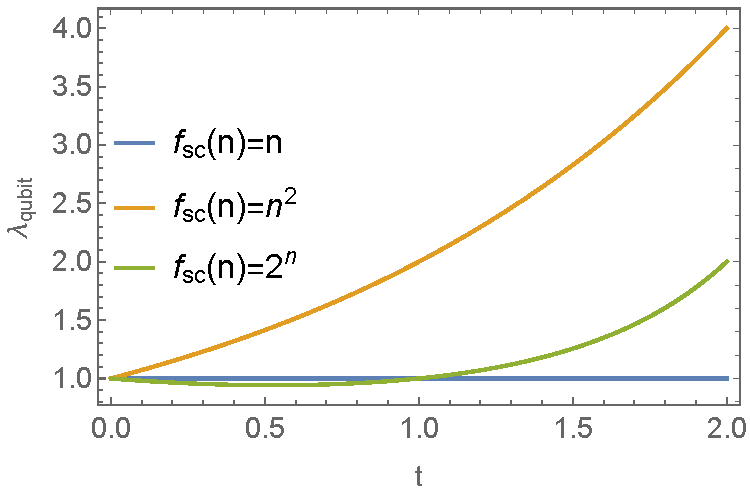
\includegraphics[width=0.42\textwidth]{single_qubit_QCL}
\caption{Time-dependent quantum computational leverage for a single qubit with different computational scaling functions, under the assumption of exponential network growth with \mbox{$N_0=1$}.}\label{fig:time_dep_QCL}
\end{figure}

%
% Forward Contract Pricing Model
%

\subsection{Forward contract pricing model}\label{sec:for_contr}\index{Forward contract pricing model}

Forward contracts are immensely useful in conventional markets, as a means by which to secure future use or ownership of an asset at predictable points in time. For example, farmers make heavy use of forward contracts to lock in sale of their produce before it has been harvested, such that the value is locked in in advance and the sale guaranteed, providing a very valuable hedging instrument\index{Hedging} for managing risk\index{Risk management}.

We envisage similar utility in the context of quantum computing. A company engaging in heavy use of computing power might have a need to perform certain computations at predictable points in the future. In this instance, forward contracts could be very helpful in reducing exposure to risk and guaranteeing access to the technology when needed, at a pre-agreed rate.

Now let us price forward contracts on qubits, whereby we wish to agree upon a price today, to be paid in the future, in exchange for ownership of qubits.

The key observation is that a unit of computation (FLOP) does not carry over time. It must be utilised immediately and cannot be stored for future use. This simplifies the forward price of a unit of computation to simply be the future spot price, discounted by the risk-free RoR, yielding the forward contract pricing model for quantum computing time-shares,
\begin{definition}[Forward contract pricing model] \label{def:forward_cont}\index{Forward contract pricing model}
The efficient market price for a forward contract in qubits is,
\begin{align}
F(T) &= e^{-r_\text{rf}T} L(T)\nonumber\\
&=\frac{e^{\gamma_\text{ror}-r_\text{rf}T} C_0{\gamma_C}^{-T}}{\chi_\text{sc}(N_0 {\gamma_N}^T)}
\end{align}
\end{definition}

Note that in the limit of \mbox{$T\to 0$} this reduces to the spot price of the asset. That is,
\begin{align}
	F(0)=L(0),
\end{align}
as expected.

\begin{figure}[!htb]
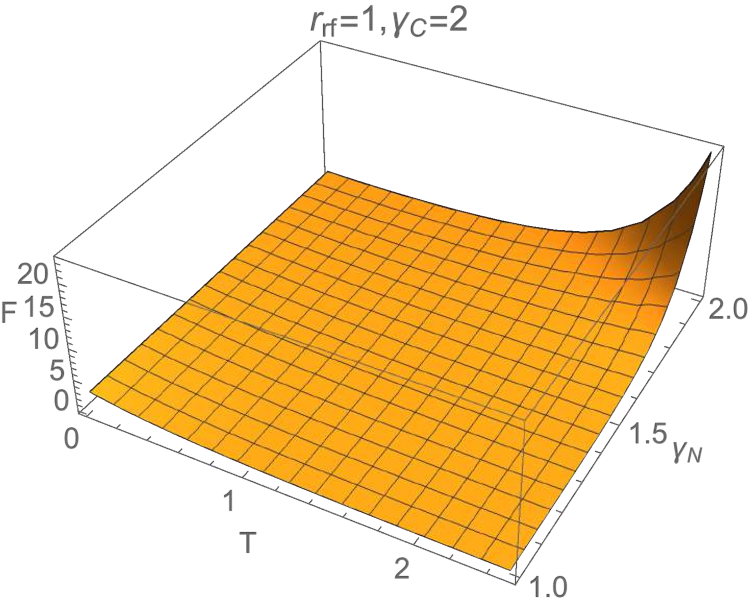
\includegraphics[width=0.4\textwidth]{forward_cont_pricing_mod_1}\\
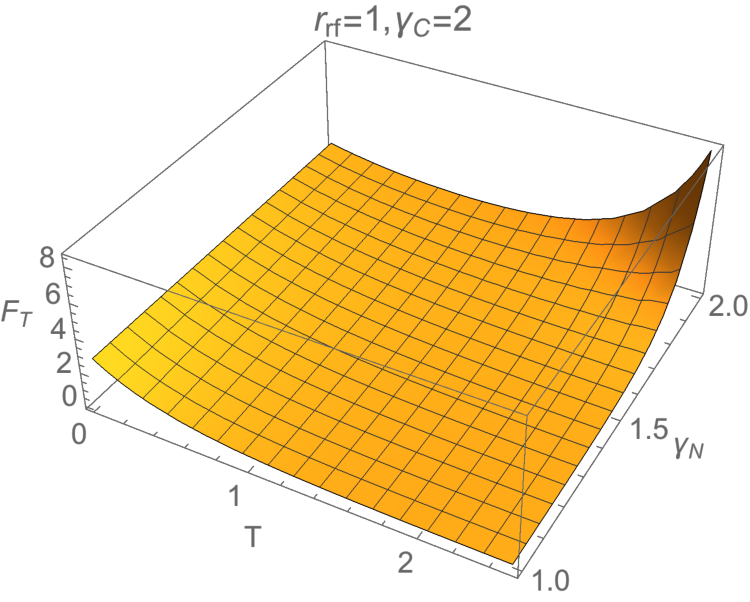
\includegraphics[width=0.4\textwidth]{forward_cont_pricing_mod_2}
\caption{Forward price on a computation to be delivered at time $T$ in the future, in units \mbox{$C_0=N_0=1$}, where we are assuming an exponential scaling function, \mbox{$f_\text{sc}(n)=e^n$}.}\label{fig:forward_cont_pricing_mod}
\end{figure}

%
% Economic Implications
%

\subsection{Economic implications}

\comment{To do}

%
% The Price To Pay For Isolationism
%

\subsubsection{The price to pay for isolationism}

\comment{To do}

\comment{Effective ratio of cost increase for isolation vs integration}

%
% Taxation
%

\subsubsection{Taxation}\label{sec:taxation}\index{Taxation}

Any asset, dividend, derivative or other financial instrument will inevitably be subject to taxation. Any form of taxation has multiplier effects as the cost markup is repeatedly handed from one market participant to the next, influencing the chain of supply and demand along the way. However, this multiplier and other economic consequences are highly dependent on the asset undergoing transaction -- the economic implications of personal income tax are quite different to those of capital gains tax.

We now consider the effect of taxation on quantum resources, specifically in the form of a \textit{qubit tax} -- a sales tax on the purchase of physical qubits. Although this model of taxation is unlikely to be implemented as we describe, it serves as an insightful test-bed for thought experiments into the qualitative implications of taxing quantum assets.

Imagine that consumers have an amount of capital available for the purchase of qubits. Let $\gamma_T$ be the rate of taxation (\mbox{$\gamma_T=1$} represents no taxation, \mbox{$\gamma_T>1$} represents positive taxation, and \mbox{$\gamma_T<1$} represents subsidisation). Then the cost of physical qubits is marked up by $\gamma_T$, reducing the number of qubits that can be afforded by the consumers to,
\begin{align}
	N_\text{tax} = \frac{N_\text{no\,tax}}{\gamma_T}.
\end{align}

We now wish to understand how this taxation influences the computational power of the network. We define the \textit{tax performance multiplier}\index{Tax performance multiplier},
\begin{definition}[Tax performance multiplier]
The \textit{tax performance multiplier}\index{Tax performance multiplier}, is the ratio between computational scaling functions with and without qubit taxation,
\begin{align}
M(N_\text{tax}) &= \frac{f_\text{sc}(N_\text{tax})}{f_\text{sc}(N_\text{no\,tax})} \nonumber \\
&= \frac{f_\text{sc}(N_\text{tax})}{f_\text{sc}(N_\text{tax} \gamma_T)},
\end{align}
where the consumers have purchased $N_\text{tax}$ qubits, after taxation, at a markup rate of $\gamma_T$.
\end{definition}
The tax performance multiplier effectively gives us a factor by which computational power is depreciated under taxation. We can accomodate for other models of taxation and regulation by choosing an appropriate relationship between $N_\text{tax}$, $N_\text{no\,tax}$, and the taxation and regulatory framework.

Using our illustrative examples of computational scaling functions (linear, polynomial and exponential), the respective tax performance multipliers are given by,
\begin{align}
M_\text{linear}(N_\text{tax}) &= \frac{1}{\gamma_T}, \nonumber \\
M_\text{poly}(N_\text{tax}) &= \frac{1}{{\gamma_T}^p}, \nonumber \\
M_\text{exp}(N_\text{tax}) &= e^{N_\text{tax}(1-\gamma_T)}.
\end{align}

This demonstrates that the computational power of classical networks is simply inversely proportional to the rate of taxation, i.e a linear tax performance multiplier, as we intuitively expect. And for quadratic scaling functions the dependence is inverse quadratic in the taxation rate. In both cases the multiplier is a constant factor, independent of the network size. However, for exponential scaling functions we observe an exponential dependence on both the rate of taxation and the size of the network, shown in Fig.~\ref{fig:tax_exp}(top). Note that for large networks, there is enormous sensitivity to variations in tax rates, yielding very high leverage in computational return by tax rates.

This implies that as the quantum network expands over time, its joint processing power decreases exponentially with the rate of taxation, yielding an ever-decreasing performance multiplier. In Sec.~\ref{sec:economics} we discuss some of the implications of this uniquely quantum phenomena.

However, taxation could also be negative, in the form of subsidisation. In Fig.~\ref{fig:tax_exp}(bottom) we focus on the region surrounding neutral taxation, showing small degrees of taxation and subsidisation on either side. Evidently, even small degrees of subsidisation have a very strong effect on the performance multiplier (more pronounced than the same rate of positive taxation!). This makes subsidisation of qubit expansion highly tempting.

\begin{figure}[!htb]
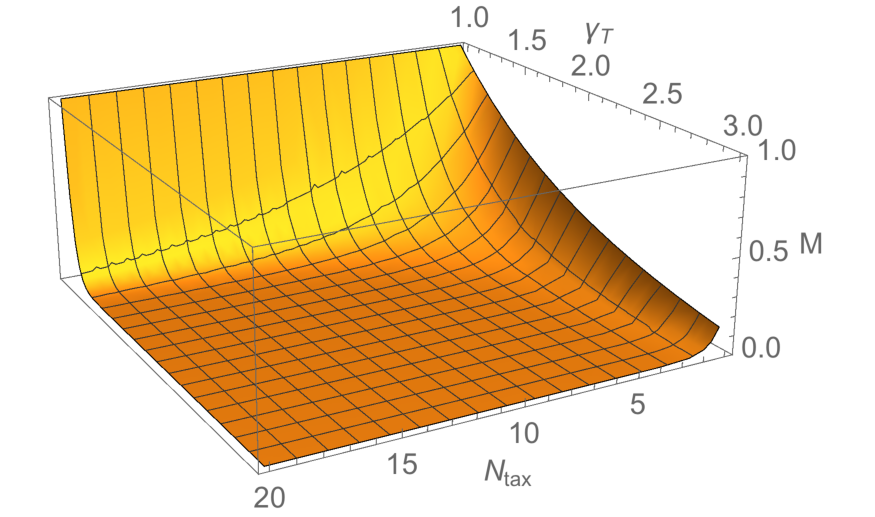
\includegraphics[width=0.47\textwidth]{tax_exp} \\
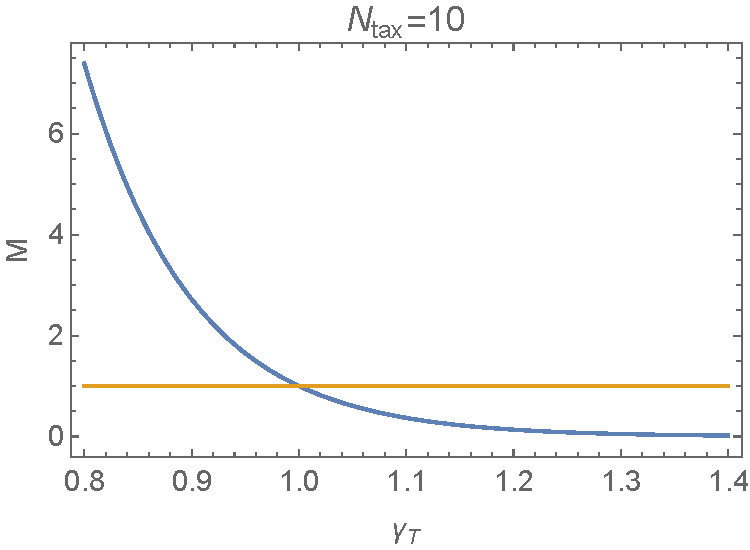
\includegraphics[width=0.47\textwidth]{tax_subsidy}
\caption{(top) Relationship between the tax performance multiplier, (positive) tax rate, and network size, assuming an exponential computational scaling function, in the regime of positive taxation, \mbox{$\gamma_T>1$}. (bottom) For \mbox{$N_\text{tax}=10$}, a zoom into the region around neutral taxation, where \mbox{$\gamma_T\approx 1$}, showing slight degrees of both taxation (\mbox{$\gamma_T>1$}) and subsidisation (\mbox{$\gamma_T<1$}). Neutral taxation, \mbox{$\gamma_T=1$}, is shown in orange.}\label{fig:tax_exp}\index{Tea party}\index{Don't tread on me}
\end{figure}

%
% Regulatory Frameworks
%

\subsubsection{Regulatory frameworks} \index{Regulatory frameworks}

\comment{To do. How will leverage asymmetry affect regulatory frameworks, defence export laws etc.}

%
% The Quantum Stockmarket
%

\subsubsection{The quantum stock market}\index{Quantum stock market}

As discussed in relation to combined computational scaling functions (Sec.~\ref{sec:comb_comp_sc_func})\index{Combined computational scaling functions}, different market participants will be executing different software applications on their share of the quantum computing resources, with differing QCLs\index{Quantum computational leverage}. Because the applications differ between users, as do their QCLs, so too does the monetary value of the computations they are performing. This yields the distinction between \textit{subjective}\index{Subjective value of computation} and \textit{objective}\index{Objective value of computation} value of computation.

The subjective value of a computation is the value to an end-user of a computation, measured in terms of their associated monetary profit from utilising its output. The objective value, rather, is the cost of the hardware, which is not application specific.

This effectively implies that some users pay more for computation (in terms of RoI\index{Return on investment}) than others. While the objective cost of computation is conceptually simple to model (as performed in a rudimentary fashion in Sec.~\ref{sec:cost_of_comp}), the subjective cost is a highly non-trivial one. It will depend heavily on the scaling function of the algorithm run by a user, and of course the economic objectives of their computation -- a quantum simulation algorithm executed by an R\&D lab\index{R\&D} is likely to be of greater monetary value than and undergrad using his university's resources for completing an assignment!

The question then is how to reconcile the distinction between subjective and objective value, given the diversity of applications in the quantum marketplace. This will supersede the na\"ive models for cost of computation presented earlier, which were based entirely on objective value. Of course, subjective value is what people are actually willing to pay for in the real-world!

This will give rise to a marketplace for tradable units of quantum computation, where the underlying asset is time-shares in the global network. We refer to this as the \textit{quantum stock market} -- a marketplace subject to ordinary supply and demand, economic, and psychological pressures. In a scenario where a large number of users are executing computations with high return (think the R\&D lab), asset values will be traded up. Contrarily, in a scenario of low-return computations (think our poor undergrad), they will be traded down. These market forces will be highly time-dependent, varying against many other factors in the economy, such as the emergence of new applications for quantum computation.

The relative market value of computation will subsequently drive the direction of investment into quantum hardware, with carry-over effects on future market prices. If investment stagnates, so too will growth in computational dividends, driving up market rates by limiting supply (assuming positive growth in demand). This will, after market adjustment, drive investment back into the system to satisfy increasing demand. Thus, despite the present uncertainty into the future dynamics of the quantum stock market, we expect this positive feedback loop to ensure consistent, ongoing investment into the quantum network, and at least some marginal degree of price stability.

What is likely to arise is that most owners of quantum hardware will not be consumers, but rather investors, who float their resources on the quantum stock market, betting on changes in demand for computation and their associated subjective cost. This trading could involve transactions in the direct underlying asset, future contracts (Sec.~\ref{sec:for_contr}) for locking in required computational power at future points in time, or more complex derivatives. For example, an investor anticipating a surge in high-value computations is likely to invest more heavily into hardware with the expectation of an uptrend in market rates. And their RoI will reflect these market dynamics.

As all markets for tradable assets do, sophisticated derivative markets will inevitably emerge, whereby people can speculate on or hedge against market dynamics, taking long, short, or more complex market positions, potentially in a highly-leveraged manner. As discussed in Sec.~\ref{sec:for_contr}, derivatives such as future contracts can be extremely helpful in enabling consumers to lock in future prices, creating a stable business climate. Similarly, other derivatives will enable market participants to hedge\index{Hedging} other quantum-related investments. For example, suppose an investor held a stake in an R\&D lab, highly reliant on quantum computing resources. By taking a leveraged long position on the market value for computation, he may limit losses on his R\&D investment associated with the higher price (and hence lower profit) they will be paying for computation.

No doubt, market manipulation and all the usual nonsense will ensue.

%
% Summary of Economic Models
%

\subsection{Summary of economic models}

In Table.~\ref{tab:summary_ec_models} we summarise the economic models and parameters we developed, and applied them to several illustrative scaling functions of particular interest: linear, polynomial, and exponential.

\renewcommand{\tablename}{TABLE}
\renewcommand{\arraystretch}{0.5}

\begin{table*}[!htb]
\begin{tabular}{|m{0.21\linewidth}|m{0.22\linewidth}|m{0.155\linewidth}|m{0.155\linewidth}|m{0.2\linewidth}|}
	\hline
	\[\text{Model}\] & \[\text{General form}\] & \[f_\text{sc}(n)=n\] & \[f_\text{sc}(n)=n^p\] & \[f_\text{sc}(n)=e^n\]\\
	\hline \hline
	\begin{flushleft}Network price scaling factor (Sec.~\ref{sec:NPSF})\end{flushleft} & \[\chi_\text{sc}(n)=\frac{f_\text{sc}(n)}{n}\] & \[1\] & \[n^{p-1}\] & \[\frac{e^n}{n}\]\\
	\hline
	\begin{flushleft}Network power (Sec.~\ref{sec:network_power})\end{flushleft} & \[P(t)=f_\text{sc}(N_0{\gamma_N}^t)\] & \[N_0{\gamma_N}^t\] & \[\left(N_0{\gamma_N}^t\right)^p\] & \[ e^{N_0{\gamma_N}^t}\] \\
	\hline
	\begin{flushleft}Network value (Sec.~\ref{sec:network_value})\end{flushleft} & \[V(t)=C_0 N_0 \left(\frac{\gamma_N}{\gamma_C}\right)^t\] & \[C_0 N_0 \left(\frac{\gamma_N}{\gamma_C}\right)^t\] & \[C_0 N_0 \left(\frac{\gamma_N}{\gamma_C}\right)^t\] & \[C_0 N_0 \left(\frac{\gamma_N}{\gamma_C}\right)^t\] \\
	\hline
	\begin{flushleft}Spot price of computation (Sec.~\ref{sec:cost_of_comp})\end{flushleft} & \[L(0)=\frac{e^{\gamma_\text{ror}} C_0}{\chi_\text{sc}(N_0)}\] & \[e^{\gamma_\text{ror}} C_0\] &  \[\frac{e^{\gamma_\text{ror}}C_0}{{N_0}^{p-1}}\] & \[\frac{e^{\gamma_\text{ror}}N_0C_0}{e^{N_0}}\] \\
	\hline
	\begin{flushleft}Future cost of computation (Sec.~\ref{sec:cost_of_comp})\end{flushleft} & \[L(t)=\frac{e^{\gamma_\text{ror}} C_0{\gamma_C}^{-t}}{\chi_\text{sc}(N_0 {\gamma_N}^t)}
\] & \[e^{\gamma_\text{ror}} C_0{\gamma_C}^{-t} \] & \[ \frac{e^{\gamma_\text{ror}} C_0{\gamma_C}^{-t}}{(N_0 {\gamma_N}^t)^{p-1}}
\] & \[ \frac{e^{\gamma_\text{ror}} C_0N_0 \left(\frac{\gamma_N}{\gamma_C}\right)^t}{e^{N_0 {\gamma_N}^t}}\] \\
	\hline
	\begin{flushleft}Time-share computational power (Sec.~\ref{sec:arb_free_time_share})\end{flushleft} & \[c_n=n \cdot \chi_\text{sc}(n_\text{global})
\] & \[n\] & \[n\cdot{n_\text{global}}^{p-1}\] & \[\frac{n e^{n_\text{global}}}{n_\text{global}}\]\\
	\hline
	\begin{flushleft}Quantum computational leverage (Sec.~\ref{sec:quant_ec_lev})\end{flushleft} & \[\lambda_n=\frac{\chi_\text{sc}(n_\text{global})}{\chi_\text{sc}(n)}\] & \[1\] & \[\left(\frac{n_\text{global}}{n}\right)^{p-1}\] & \[\frac{n e^{n_\text{global}}}{n_\text{global}e^n}\]\\
	\hline
	\begin{flushleft}Single-qubit leverage (Sec.~\ref{sec:quant_ec_lev})\end{flushleft} & \[\lambda_\text{qubit}=\frac{\chi_\text{sc}(n_\text{global})}{\chi_\text{sc}(1)}\] & \[1\] & \[{n_\text{global}}^{p-1}\] & \[\frac{e^{n_\text{global}-1}}{n_\text{global}}\]\\
	\hline
	\begin{flushleft}Time-dependent leverage (Sec.~\ref{sec:quant_ec_lev})\end{flushleft} & \[\lambda_n(t)=\frac{\chi_\text{sc}(N_0{\gamma_N}^t)}{\chi_\text{sc}(n)}\] &  \[1\] & \[\left(\frac{N_0{\gamma_N}^t}{n}\right)^{p-1}\] & \[\frac{n e^{N_0{\gamma_N}^t-n}}{N_0{\gamma_N}^t}\]\\
	\hline
	\begin{flushleft}Forward contract price (Sec.~\ref{sec:for_contr})\end{flushleft} & \[F(T)=\frac{e^{\gamma_\text{ror}-r_\text{rf}T} C_0{\gamma_C}^{-T}}{\chi_\text{sc}(N_0 {\gamma_N}^T)}\]
 & \[e^{\gamma_\text{ror}-r_\text{rf}T} C_0{\gamma_C}^{-T}\] & \[\frac{e^{\gamma_\text{ror}-r_\text{rf}T} C_0{\gamma_C}^{-T}}{(N_0 {\gamma_N}^T)^{p-1}}\] & \[\frac{e^{\gamma_\text{ror}-r_\text{rf}T} C_0N_0\left(\frac{\gamma_N}{\gamma_C}\right)^T}{e^{N_0 {\gamma_N}^T}}\] \\
	\hline
	\begin{flushleft}Tax performance multiplier (Sec.~\ref{sec:taxation})\end{flushleft} & \[M(N_\text{tax})=\frac{f_\text{sc}(N_\text{tax})}{f_\text{sc}(N_\text{tax} \gamma_T)}\] & \[\frac{1}{\gamma_T}\] & \[\frac{1}{{\gamma_T}^p}\] & \[e^{N_\text{tax}(1-\gamma_T)}\]\\
	\hline
\end{tabular}
\caption{Summary of the dynamics of various economic models under several computational scaling functions ($f_\text{sc}$) of interest, where there are $n$ qubits held by the respective node and \mbox{$n_\text{global}=\sum_{j\in \text{nodes}} n_j$} qubits in the global network. $N_0$ is the initial number of qubits, undergoing growth rate $\gamma_N$. $C_0$ is the initial monetary cost per qubit, undergoing decay rate $\gamma_C$. $\gamma_\text{ror}$ is the rate of return on the licensing of compute-time on qubits, and $r_\text{rf}$ is the risk-free rate of return. $\gamma_T$ is the rate of taxation, and $N_\text{tax}$ is the number of qubits that would exist on the network in the absence of taxation.} \label{tab:summary_ec_models}
\end{table*}

\renewcommand{\arraystretch}{1}
\renewcommand{\tablename}{ALG.}

\clearpage